\documentclass[letterpaper,12pt]{article}
\usepackage{tabularx} % extra features for tabular environment
\usepackage{amsmath}  % improve math presentation
\usepackage{float}
\usepackage{pdfpages}

\usepackage{multicol}
\usepackage{graphicx} % takes care of graphic including machinery
\graphicspath{ {./figures/} }
%\usepackage[margin=1in,letterpaper]{geometry} % decreases margins
%\usepackage{cite} % takes care of citations
\usepackage[final]{hyperref} % adds hyper links inside the generated pdf file
\hypersetup{
	colorlinks=true,       % false: boxed links; true: colored links
	linkcolor=blue,        % color of internal links
	citecolor=blue,        % color of links to bibliography
	filecolor=magenta,     % color of file links
	urlcolor =blue         
}
\usepackage[margin = 1in,headsep=0.5cm,headheight=2cm,letterpaper]{geometry} 

\usepackage{fancyhdr}
\pagestyle{fancy}
\lhead{Student 1 : Ahmet Akman 2442366 \\ Student 2: Yusuf Toprak Yıldıran 2444149 \\ Assistant: Onur Selim Kılıç}
\rhead{Date: \today \\ Group: Wednesday Morning - 5} 
%\cfoot{center of the footer!}
\renewcommand{\headrulewidth}{0.1pt}



\begin{document}
\thispagestyle{empty}

\title{Spring 2022 EE214 Experiment 6  \protect\\ Frequency Response}
\author{Ahmet Akman 2442366 \protect\\ Yusuf Toprak Yıldıran 2444149 \protect\\ Assistant: Onur Selim Kılıç}
\date{\today}
\maketitle
\tableofcontents
%\begin{abstract}
%abstract
%\end{abstract}
\section{Introduction}

\section{Experimental Results and Discussion}
The results of the experiment are discussed in the following steps.
%
\subsection{Step 1}
In this step, circuit given in Figure 1 is set with its settings and sine wave of 10V peak is adjusted.
\begin{figure}[H]
    \centering
    \includegraphics[width = 0.75\textwidth]{{highpass.png}}
    \caption{Circuit schematic for step 1}
\end{figure} 
\subsubsection{a.}
For this part, half-power angular frequency is determined by changing the input frequency manually untill obsetving \(V_0\) equals to 0.7 times of input voltage, and cutoff frequency(half-power frequency) is found as approximately 500Hz.
\subsubsection{b.}
For this part, magnitude and phase responses of the circuit in Figure 1 are obtained by using the BenchVue test flow. In order to do this,
\begin{itemize}
    \item Agilent Signal Generator and oscilloscope are intialized with 20V pp.
    \item Test flow is constructed by using sweep option from \(\frac{f_c}{5}\)(half-power frequency/5) to \(5f_c\) with \(\frac{f_c}{5}\) steps.
    \item After running the test, magnitude vs frequeny plot is obtained. 
    \item Then, data is imported to MATLAB and magnitude and phase response plots are obtained by indicating the cutoff frequency in te plot.
\end{itemize}
To obtain magnitude ch2 voltage measurement vector is divided by ch1 voltage measurement vector by pairwise(using ./) and magnitude response is plotted as magnitude in the y axis and frequency measurement is in the x axis in Figure 2.
\begin{figure}[H]
    \centering
    \includegraphics[width = 0.75\textwidth]{{1_1_1.png}}
    \caption{Magnitude response of circuit 1}
\end{figure} 
To obtain phase response a plot in which mod(phase-measurement+180,360)-180 is in the y axis and frequency measurement vector is in the x axis is obtained in Figure 3.
\begin{figure}[H]
    \centering
    \includegraphics[width = 0.75\textwidth]{{1_1_2.png}}
    \caption{Frequency response of circuit 1}
\end{figure} 
Since high pass filter allows frequencies that greater than the cutoff frequency to pass, by looking at the magnitude response it can be said that this filter is highpass filter.
\subsection{Step 2}
\subsection{Step 3}
\subsection{Step 4}
In this step, circuit in Step 3 is used.
\subsubsection{a.}
For this step, a square wave at the resonant frequency where magnitude response is equal to 1 is applied and then input and output voltages are plotted in figure x.
Since this pircuit passes some frequency interval to pass it is called bandpass filter.  
\begin{figure}[H]
    \centering
    \includegraphics[width = 0.75\textwidth]{{STP4ct.png}}
    \caption{Frequency response of circuit 1}
\end{figure} 
\subsubsection{b.}
For this step, circuit in figure x is set and a sine wave at the resonant frequency is applied. Then, \(V_{01}\) and \(V_{02}\) plot is obtained in Figure x.
\begin{figure}[H]
    \centering
    \includegraphics[width = 0.75\textwidth]{{STP4ct.png}}
    \caption{Frequency response of circuit 1}
\end{figure} 

\begin{figure}[H]
    \centering
    \includegraphics[width = 0.75\textwidth]{{STP4ct.png}}
    \caption{Frequency response of circuit 1}
\end{figure} 
Since there is a capacitor at the load, capacitor discharges in the negative cycle of the input. Therefore, \(V_{01}\) is measured as sine wave while \(V_{02}\) is 0 at the negative cycle.
\section{Conclusion}



\section*{Appendix A}
\begin{itemize}
    \item PreLab Preparation 3 hours
    \item Experimental Work 2  hours
    \item Report Writing 8 hours
\end{itemize}
\section*{Appendix B}
In this experiment, since the values the students obtained in the lab is quite close to the data provided by the lab assistants, it is preffered to use the data obtained by the students.

\end{document}

%%%%%%%%%%%%%%%%%%%%%%   EXAMPLE TABLE   %%%%%%%%%%%%%%%%%%%%%%%%%%%%%%%%
\begin{table}[H]
\begin{center}
    \caption{Resistance reading by color code convention.}
    \vspace{2mm}
    \begin{tabular}{||c | c | c||} 
        \hline
        Color Order & Value & Tolerance \\ [0.5ex] 
        \hline\hline
        Brown / Black / Red / Gold & 1k\( \Omega \) & \( \% \) 5  \\ 
        \hline
        Yellow / Violet / Red / Gold & 4.7k\( \Omega \) & \( \% \) 5   \\
        \hline
        Brown / Grey / Orange / Gold & 18k\( \Omega \) & \( \% \) 5  \\ [1ex] 
        \hline
    \end{tabular}
\end{center}
\end{table}


%%%%%%%%%%%%%%%%%%%%%%   EXAMPLE IMAGE   %%%%%%%%%%%%%%%%%%%%%%%%%%%%%%%%
\begin{figure}[H]
\centering
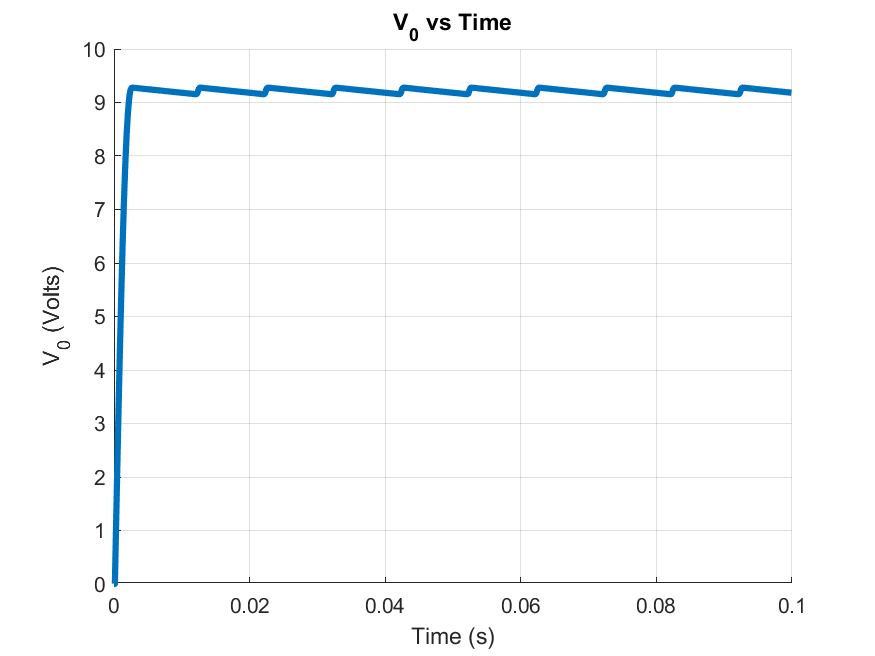
\includegraphics[width = 0.75\textwidth]{5.png}
\caption{Circuit schematic for the step 5}
\end{figure} 

%%%%%%%%%%%%%%%%%%%%%%   EXAMPLE IMAGE FROM PDF   %%%%%%%%%%%%%%%%%%%%%%%%%%%%%%%%
\begin{figure}[H] \centering{
	\includegraphics[scale=0.25]{2a_plot.pdf}}
	\caption{Experiment 2}
\end{figure}
%%%%%%%%%%%%%%%% Deneme Push